\documentclass[11pt]{article}
\usepackage[letterpaper]{geometry}

%Used to split pages into two columns, IE the truth tables
\usepackage{multicol}

%Used to place figures
\usepackage{graphicx}
\usepackage{float}

%Used so that multi-line caption text is centered instead of left-aligned
\usepackage[center]{caption}

%Used to squish TOC
\usepackage{setspace}

%Used to show code nicely formatted
\usepackage{listings}
\usepackage{color}
\usepackage{placeins}

%Used for Showing Mathematical Proofs
\usepackage{amsmath,amsthm,amssymb}

%Used for tables
\usepackage{array}
\usepackage{booktabs}

%Used for canceling terms in Math
\usepackage{cancel}

\usepackage{enumitem}

%Used to strike out items
\usepackage[normalem]{ulem}

\definecolor{dkgreen}{rgb}{0,0.6,0}
\definecolor{gray}{rgb}{0.5,0.5,0.5}
\definecolor{mauve}{rgb}{0.58,0,0.82}

\lstset{frame=tb,
	language=Java,
	aboveskip=3mm,
	belowskip=3mm,
	showstringspaces=false,
	columns=flexible,
	basicstyle={\small\ttfamily},
	numbers=none,
	numberstyle=\tiny\color{gray},
	keywordstyle=\color{blue},
	commentstyle=\color{dkgreen},
	stringstyle=\color{mauve},
	breaklines=true,
	breakatwhitespace=true,
	tabsize=3
}

%Used to include the signatures sheet
\usepackage{pdfpages}

\title{EENG-331 Lab 5:\linebreak \linebreak CS stage Design and Audio Processing}
\author{Jeremy Munson}
\geometry{top=.8in, bottom=.8in, left=.8in, right=.8in}

\setlength{\parindent}{0em}
\setlength{\parskip}{.5em}
\setlength{\floatsep}{20px}
\setlength{\textfloatsep}{20px}

\begin{document}
    \null \hfill May 18, 2024\linebreak
    \null \hfill Jeremy Munson\linebreak
    \null \hfill Corbin Cole\linebreak
    
    \makebox[\textwidth]{\textbf{\huge EENG-331 Lab 5:}}

    \makebox[\textwidth]{\textbf{\large CS stage Design and Audio Processing}}
    \vspace{-20px}
	\section{Prelab}
		\FloatBarrier
		\vspace{-5px}
	
	\subsection{Common Source Amplifier With Resistor Biasing and Passive Load}
		Prior to the lab, each team member designed a Common Source Stage with resistor divider biasing and resistor load, for $A_v = 10$, $5mW$ power budget, $V_{ov} = 100mV$, $k_p = \frac{100\mu A}{V^2}$, $V_{dd} = 5V$, $\lambda = 0$, and $V_{th} = 0.5V$. Additionally, it was assumed that an "investment" of 10\% of the power budget on setting the gate voltage was intended. Finally, we assumed that $L = 10\mu m$ is the smallest allowable value for the design. The hand-calculations for this amplifier design can be seen in Figure(\ref{fig:prelab1}). The resulting design has values as follows:\\
		\begin{align}
			\label{eqn:CS_POW_ID} &P_{\text{ower consumed by } I_d} = 90\% \cdot 5mW &=& 4.5mW \\
			\label{eqn:CS_ID} &I_d = \frac{4.5mW}{5v} &=& 0.9mA \\
			\label{eqn:CS_WL} I_d = 0.9mA = \frac{1}{2} k_p \frac{W}{L} V_{ov}^2 \rightarrow &\frac{W}{L} &= \frac{18000\mu}{10\mu} =& 1800 \\
			\label{eqn:CS_gm} &g_m = \frac{2I_d}{V_{ov}} &=& 18mS \\
			\label{eqn:CS_RD} A_v = -g_mR_d \rightarrow |A_v| = g_mR_d \rightarrow &R_d &=& 556_\Omega \\
			\label{eqn:CS_VG} &V_{g,dc} = V_{th} + V_{ov} &=& 0.6v \\
			\label{eqn:CS_GATE_BIAS} &I_{\text{gate voltage divider}} = \frac{10\% \cdot 5mW}{5v} &=& 0.1mA \\
			\label{eqn:CS_R2} &R_2 = \frac{0.6V}{0.1mA} &=& 6k_\Omega \\
			\label{eqn:CS_R1} &R_1 = \frac{5V - 0.6V}{0.1mA} &=& 44k_\Omega
		\end{align}

	\subsection{Common Source Amplifier With Self-Biasing, Active Load}
		Additionally, a CS stage was designed using a current source for the load, and the self-biasing method for setting the gate voltage. This stage follows all the same constraints as the previous section.
		
		Regarding $I_d$, the instructions say to use the same $I_d$ as the previous stage. This would be only $0.9mA$, and also did not seem to be in alignment with email communications received about the lab calculations. We instead chose to interpret this as "Use the same power budget", which results in $I_d = 1mA$, and is consistent with the other communications received.
		
		Before presenting the calculations, know that an oversight was made on the gain of the stage initially, but quickly corrected after the start time of the lab. Since the prelab was due at the start of the lab, we present the initial flawed calculations in the scan of the prelab, but the correct calculations in this lab report. The flawed calculations can be seen in Figure(\ref{fig:prelab2}).
		
		The mistake made was to take the gain equation for CS w/ active load, $A_v = g_m r_o$, and use it with $\lambda = 0$, but mistakenly behave as if \cancel{$r_o = 1$} in that case, which gave \cancel{$A_v = g_m$}, suggesting a need for a very large $g_m$. It is believed that a contributing factor to the mistake was the nonsensical correct result: $r_o = \infty$, which is fine, but $A_v = g_m \cdot \infty = \infty$, which would make it impossible to meet the $A_v = 10$ constraint.
		
		The calculations for this stage are much more simple. Self-biasing will set $V_g$. We simply need to choose $\frac{W}{L}$ such that $V_{ov} = 0.1$, to match the constraint. We take Equation(\ref{eqn:CS_WL}), and recalculate $\frac{W}{L}$ for $I_d = 1mA$, returning Equation(\ref{eqn:SB_WL}).
		\begin{align}\label{eqn:SB_WL} I_d = 1mA = \frac{1}{2} k_p \frac{W}{L} V_{ov}^2 \rightarrow \frac{W}{L} = \frac{20000\mu}{10\mu} = 2000 \end{align}
		
		
		The choice of $R_g$ is arbitrary, but it is worth noting that $R_g$ results in coupling between $V_{in}$ and $V_{out}$. Since a CS stage is an inverting amplifier, this makes the coupling a negative feedback to the input, degrading our overall gain. In our simulations we are using a voltage source with no series resistance for $V_{in}$; as a result this effect is not seen except as an interaction with the input coupling capacitor, which we can suppress by making the capacitor arbitrarily large.
		
	\begin{figure}
		\centering
		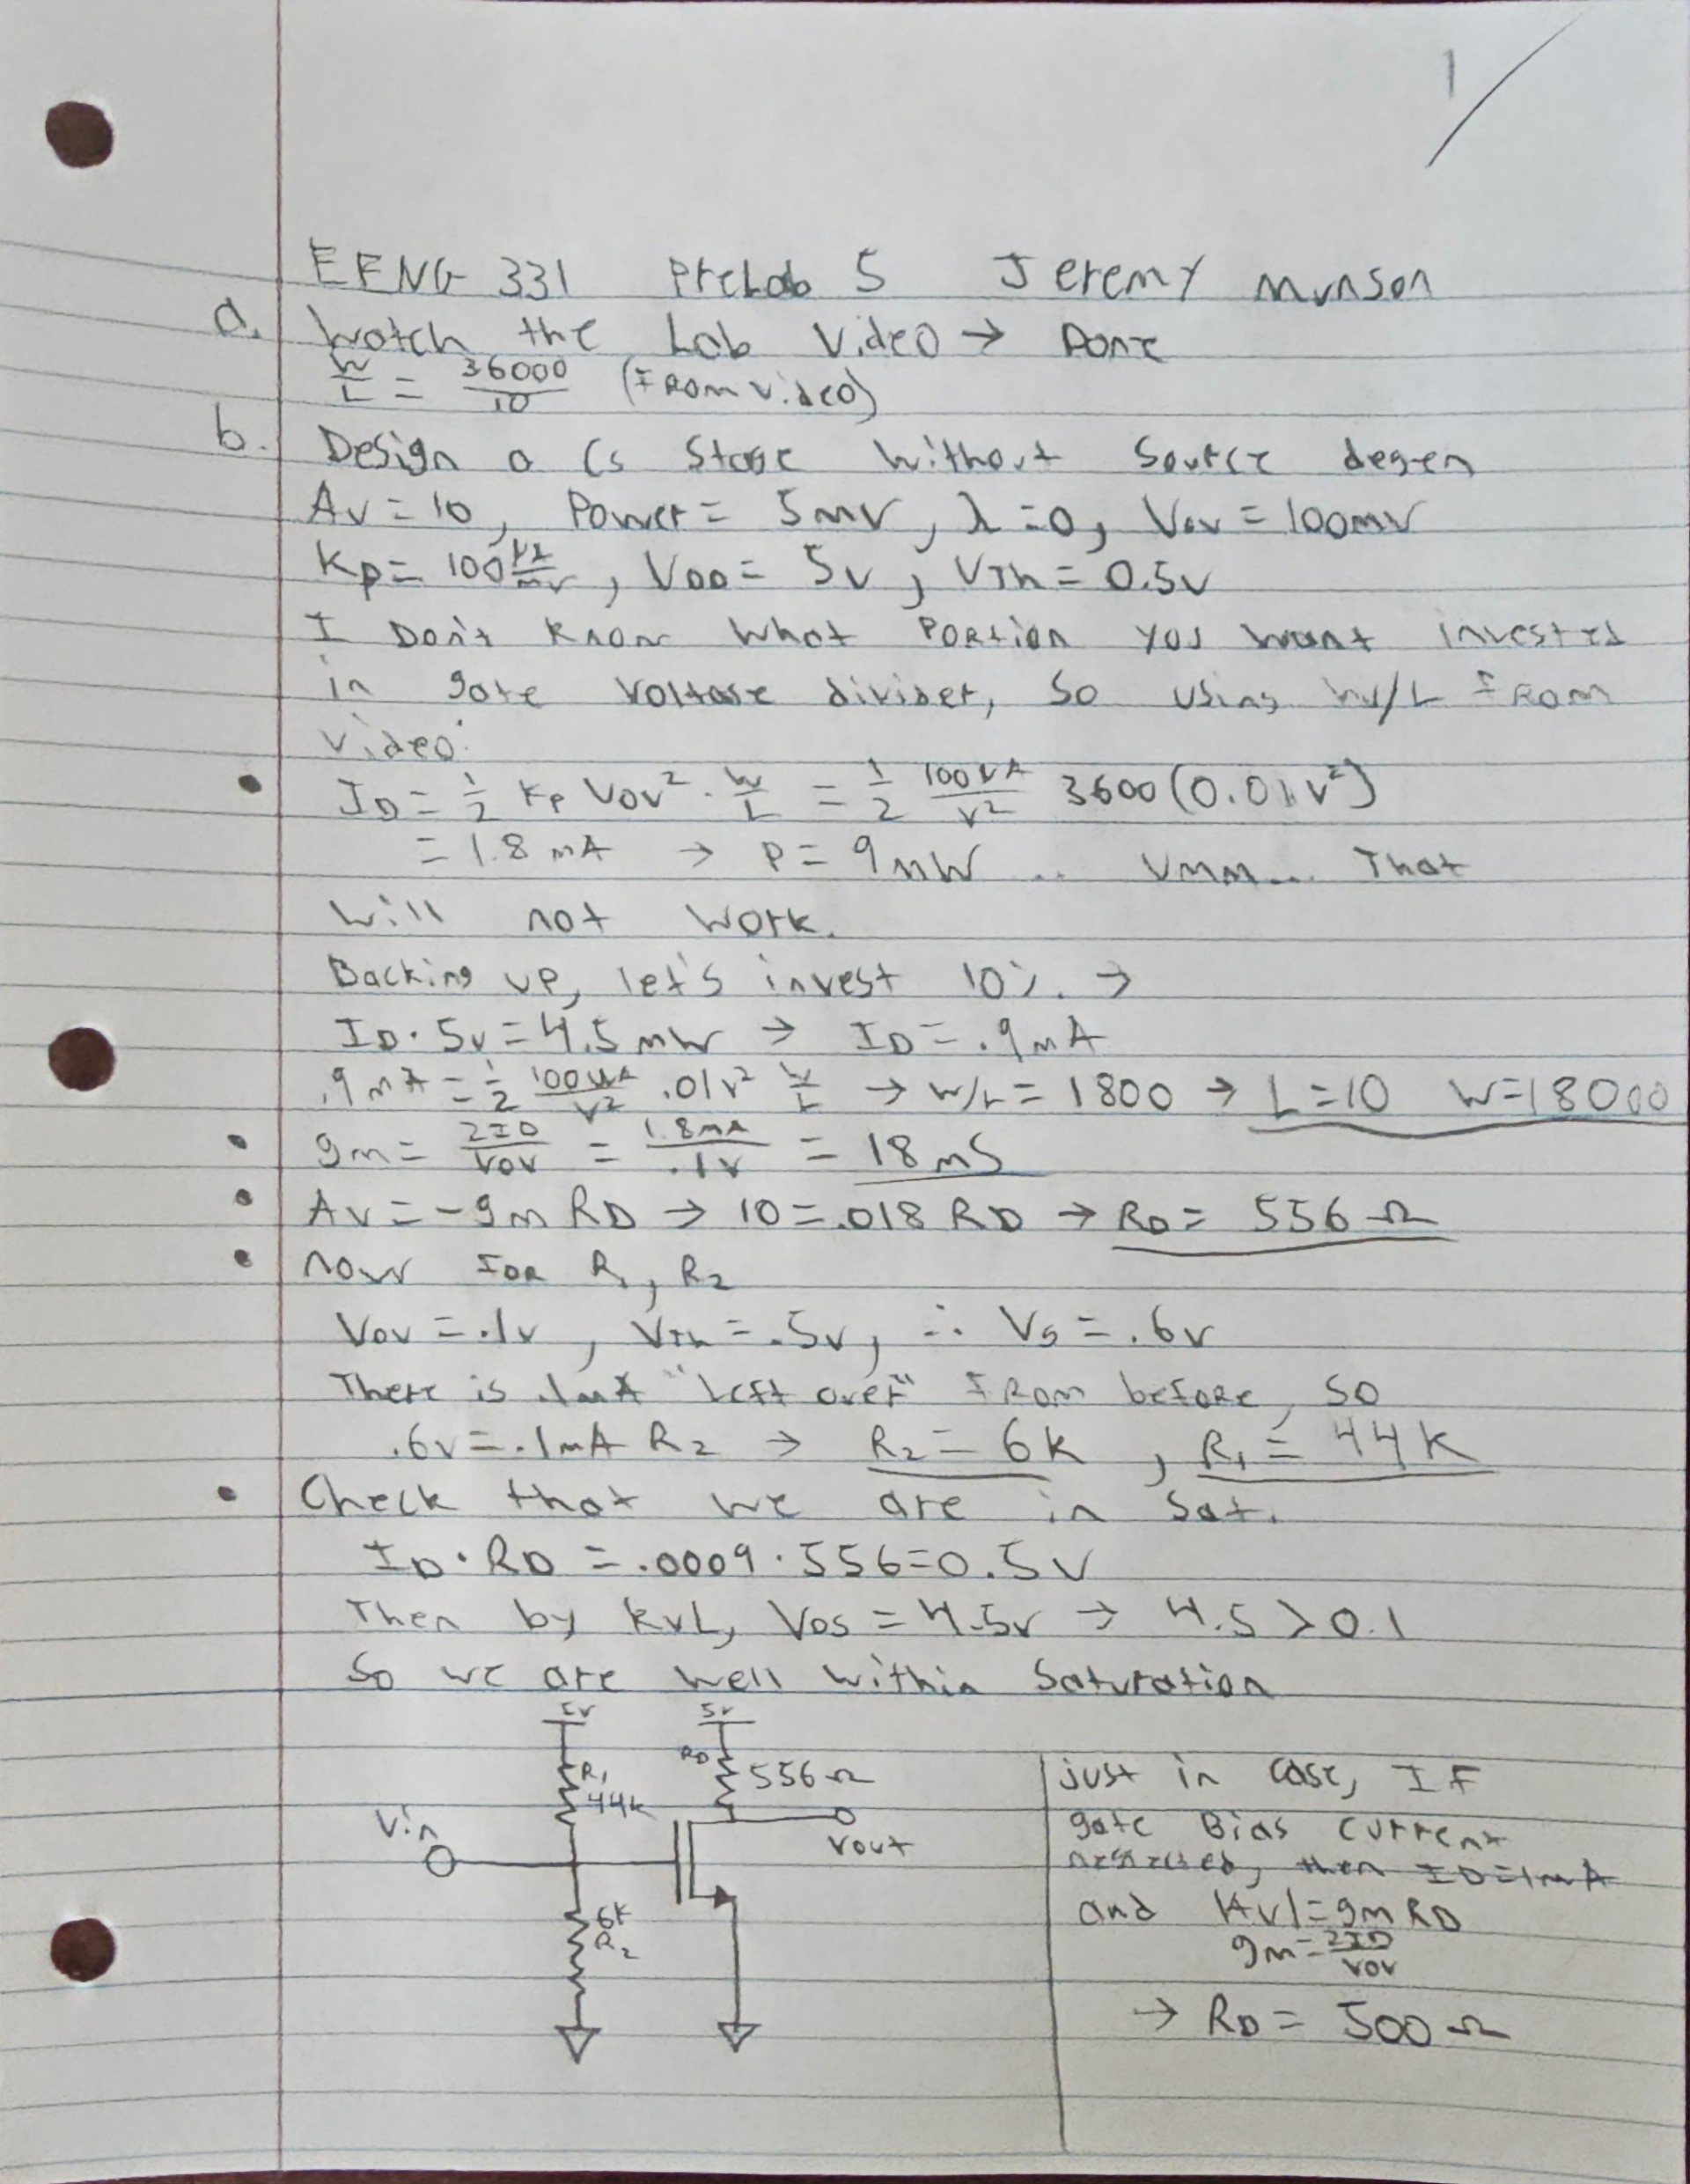
\includegraphics[width=0.95\linewidth]{prelab1}
		\caption{Prelab Calculations for CS amplifier with resistor load \& biasing}
		\label{fig:prelab1}
	\end{figure}

	\begin{figure}
	\centering
		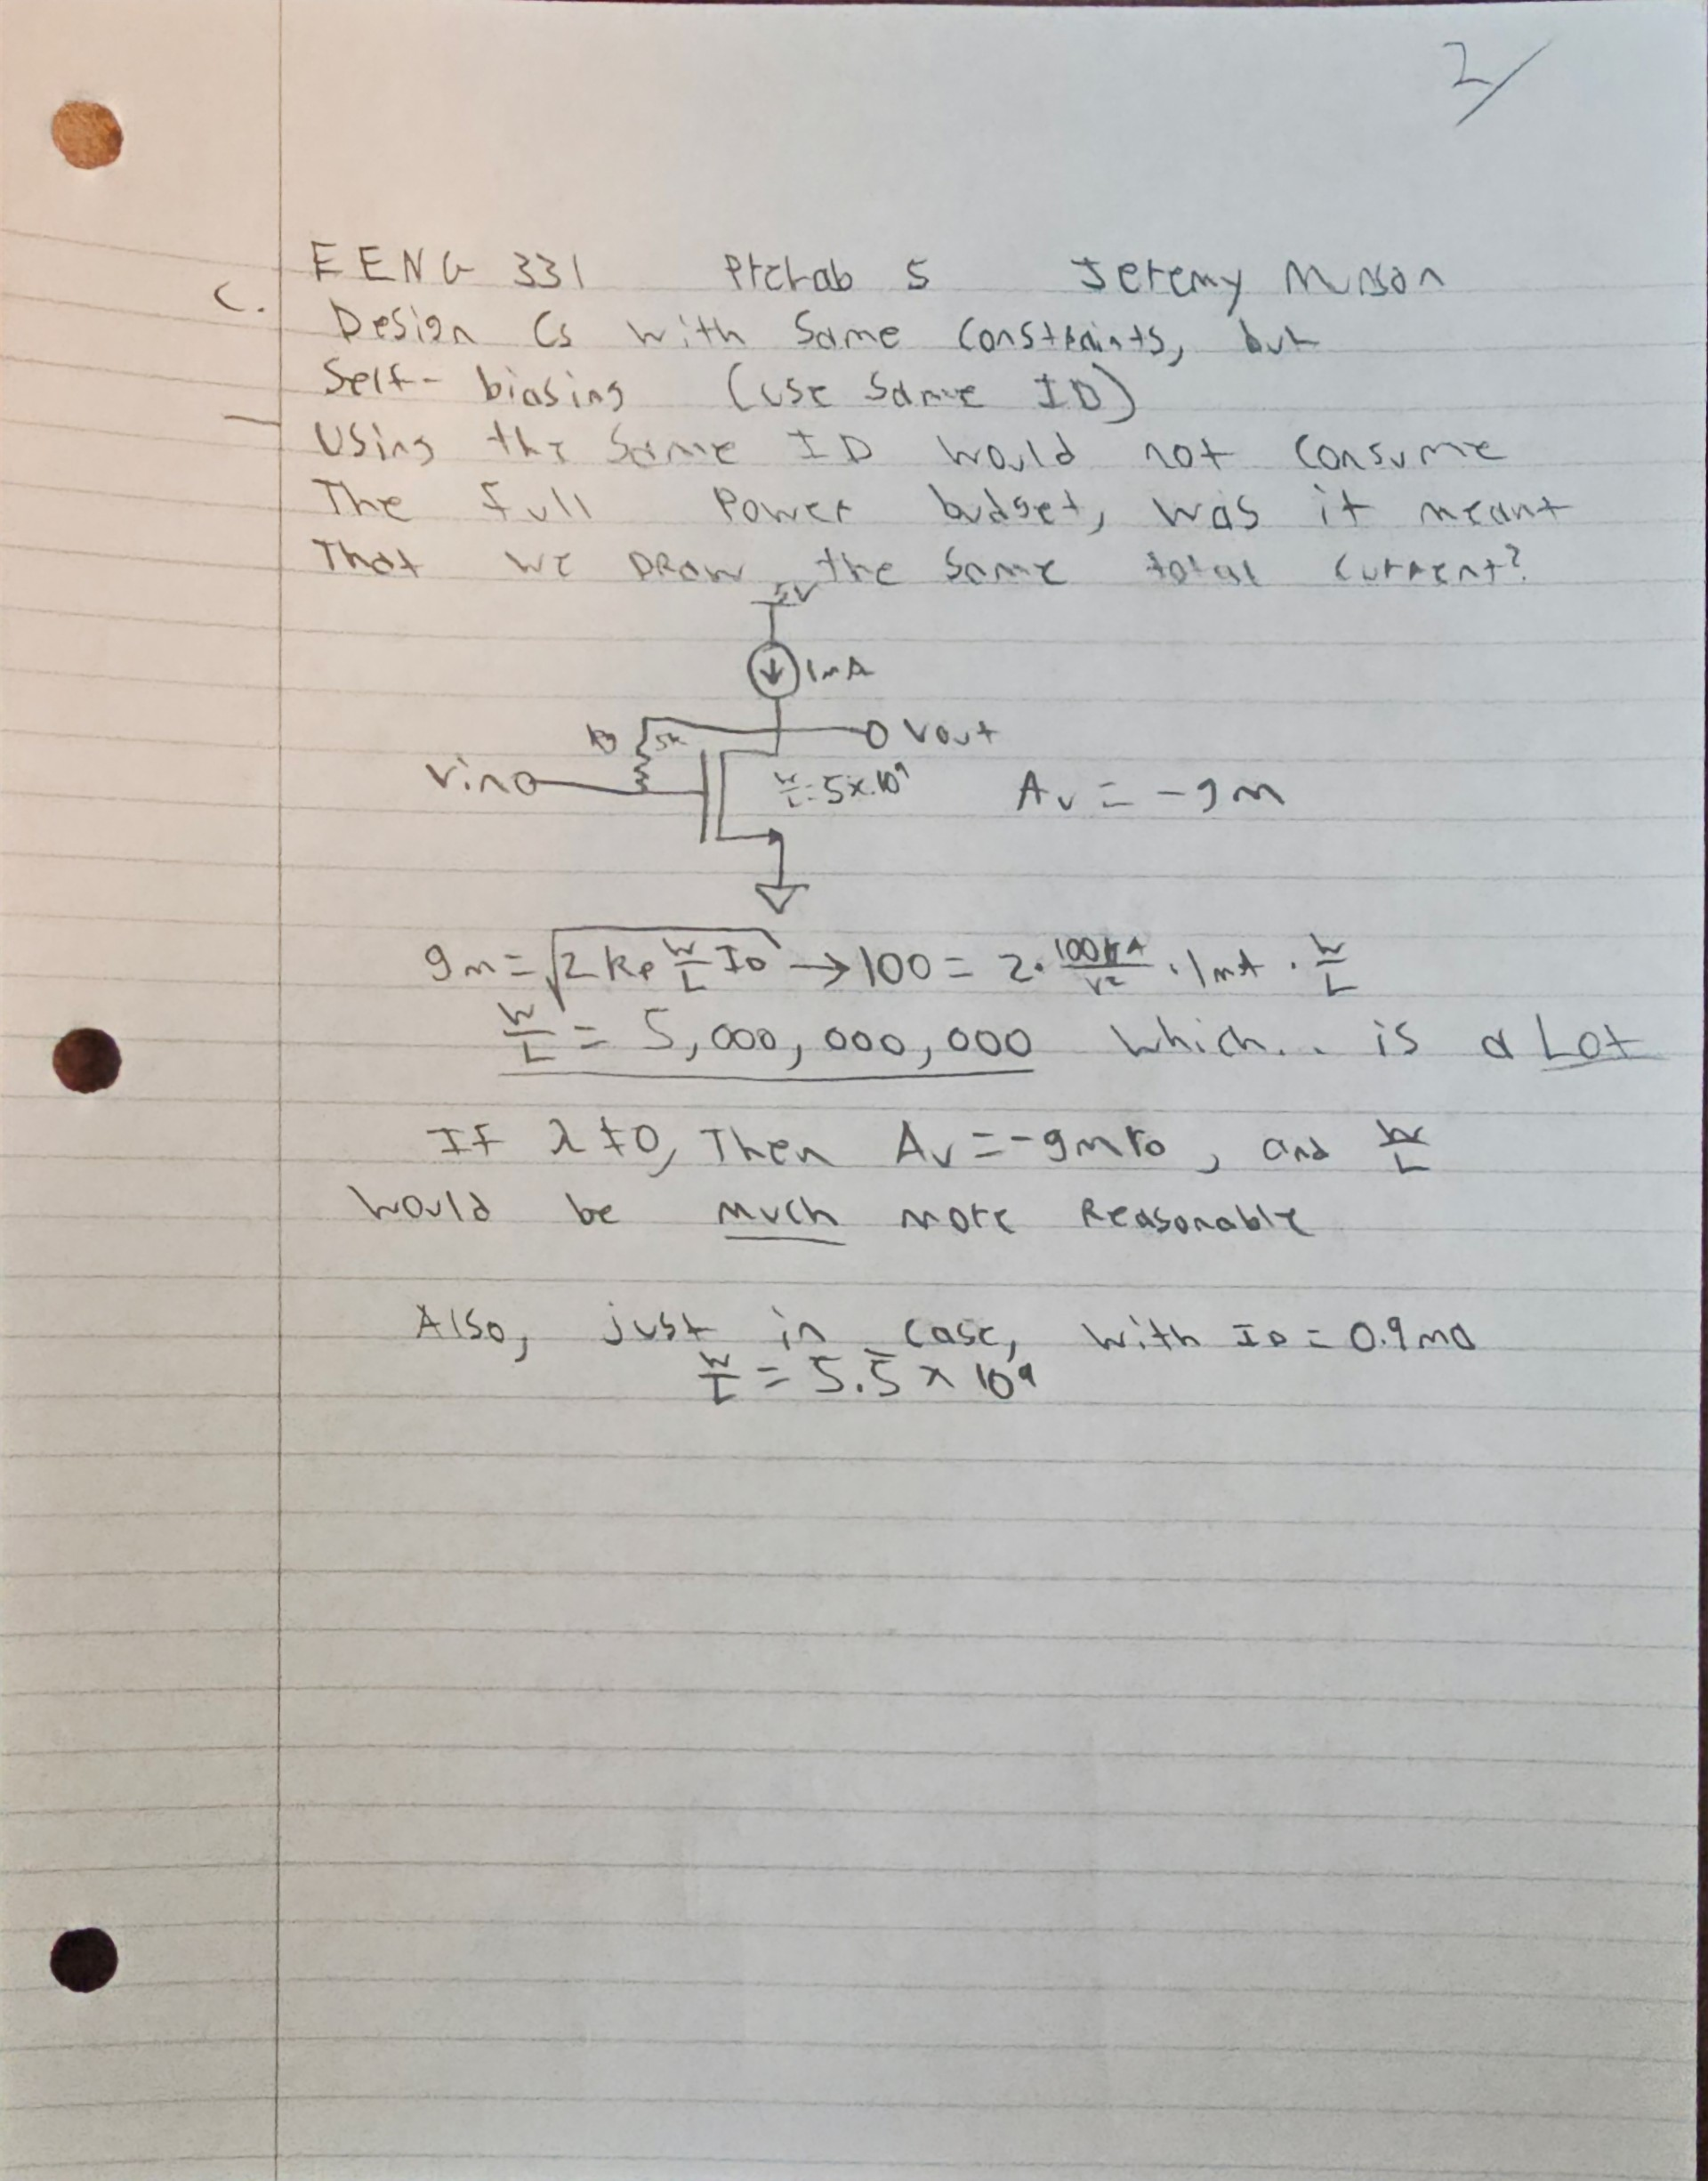
\includegraphics[width=0.95\linewidth]{prelab2}
		\caption{Mistaken Prelab Calculations for CS amplifier w/ active load and self-biasing}
		\label{fig:prelab2}
	\end{figure}

\FloatBarrier

	\section{Task 1}
	
	\subsection{Parts a,b: Plot and Attenuate Harvey Super Cool, Save output to file}
	
		\subsubsection{Tasks}
		\begin{itemize}
			\item Import a .wav file into LTSpice and use it as a voltage source.
			\item Attenuate the signal by a factor of $\frac{1}{201}$ using a voltage divider. 
			\item Plot the waveform before and after attenuation.
			\item Save the resulting attenuated waveform to a file.
		\end{itemize}
	
		\subsubsection{Calculations}
		In order to attenuate the signal with a voltage divider, we must calculate the values of the resistors in the divider. Only the ratio matters for this, not the magnitudes. For this reason, the convenient value of $R_2 = 1\Omega$ is chosen. This is shown in Equation(\ref{eqn:T1_PA_R}).
		\begin{align} \label{eqn:T1_PA_R} \frac{1}{201} = \frac{R_2}{R_1 + R_2} \rightarrow R_1 = 200_\Omega, R_2 = 1_\Omega\end{align}
	
		\subsubsection{Description, Observation}
			We prepared the LTSpice schematic according to the lab instructions and prelab video, as can be seen in Figure(\ref{fig:T1_PA_SCHEMATIC}). Here $V_1$ is a voltage source using the input .wav file, $R_1$ and $R_2$ form the voltage divider for attenuation, wav\_attenuated is the name of the net at the output of the voltage divider, and we add in an additional spice directive, .wave, which instructs LTSpice to save the specified raw data as a .wav file with a particular name, bit depth, and sample rate.
			
			We ran the simulation with the transient analysis settings specified in the lab document, and plot the input and attenuated output, resulting in the plots of Figure(\ref{fig:T1_PA_RESULT}). It can be seen that the maximum voltage swing on the input waveform is $\pm1V$ while the output waveform appears to be $\pm5mV$. Measurement of the waveform in LTSpice (not shown) shows the attenuated waveform has an actual full-scale voltage of $\approx \pm 4.975mV$.
			
			After running the transient analysis, a file is created from the attenuated output. We played this file using an audio player, as can be seen in Figure(\ref{fig:T1_PA_PLAYER}). The resulting audio was very quiet, and we had to turn the computer audio up to "150\%" to hear it. Turning the volume up this high did not cause any audio clipping or artifacts that were observed.
			
		\subsubsection{Analysis}
			The voltage divider worked exactly as expected, as seen in Figure(\ref{fig:T1_PA_RESULT}). The associated waveform measurements confirmed our attenuation by a factor of $\frac{1}{201}$. Playing the audio file that was exported also confirmed that the audio was successfully attenuated. We can also see that, since there was no observed clipping or distortion in the sound played afterwards when the computer volume was turned up past $100\%$, that the signal is indeed attenuated.
	
	\begin{figure}[h]
		\centering
		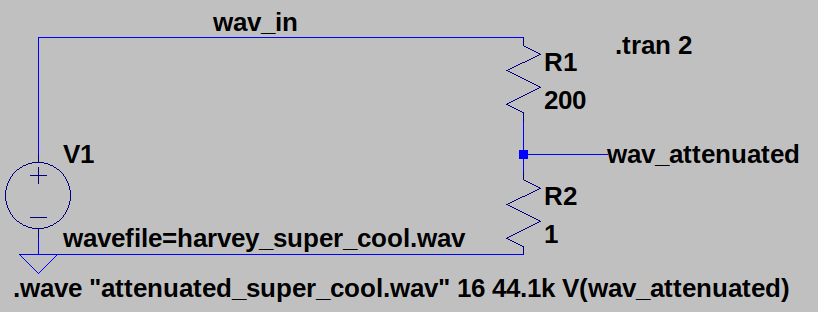
\includegraphics[width=0.85\linewidth]{task_1_ab_schematic}
		\caption{LTSpice schematic for a the .wav file import, voltage divider attenuation, and export}
		\label{fig:T1_PA_SCHEMATIC}
		\vspace{1mm}
	\end{figure}

	\begin{figure}[h]
		\centering
		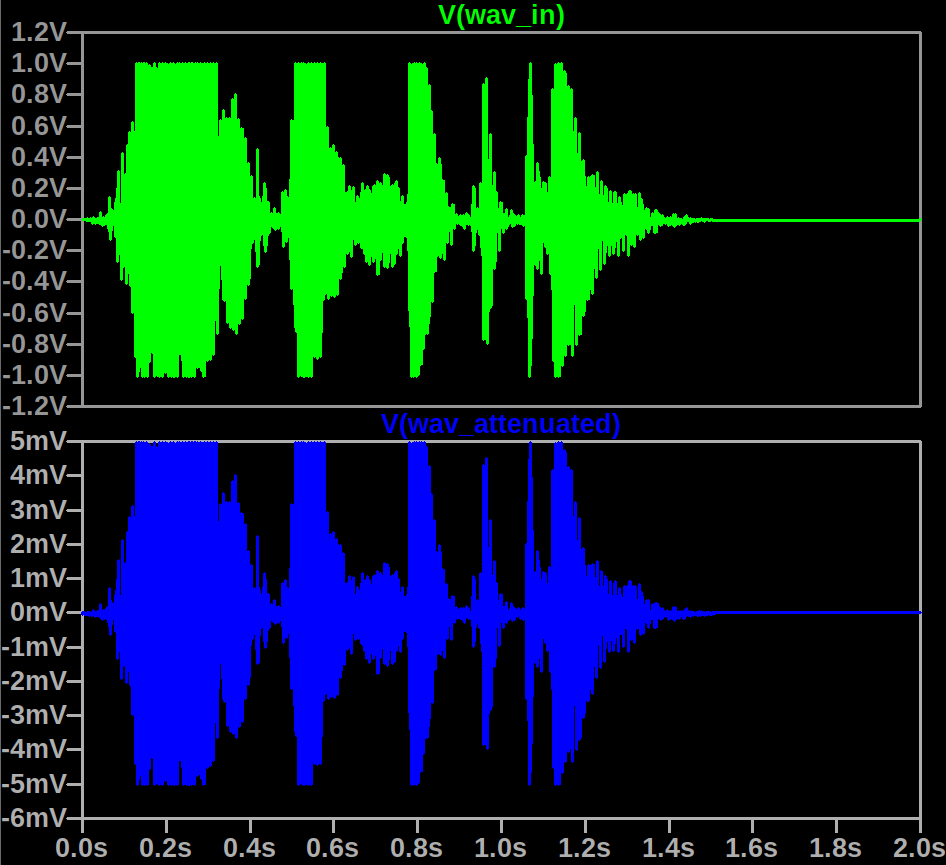
\includegraphics[width=0.85\linewidth]{task1_a_wav_before_and_after}
		\caption{Plots comparing the input Harvey Super Cool audio, and the attenuated output waveform.}
		\label{fig:T1_PA_RESULT}
		\vspace{1mm}
	\end{figure}
	
	\begin{figure}[h]
		\centering
		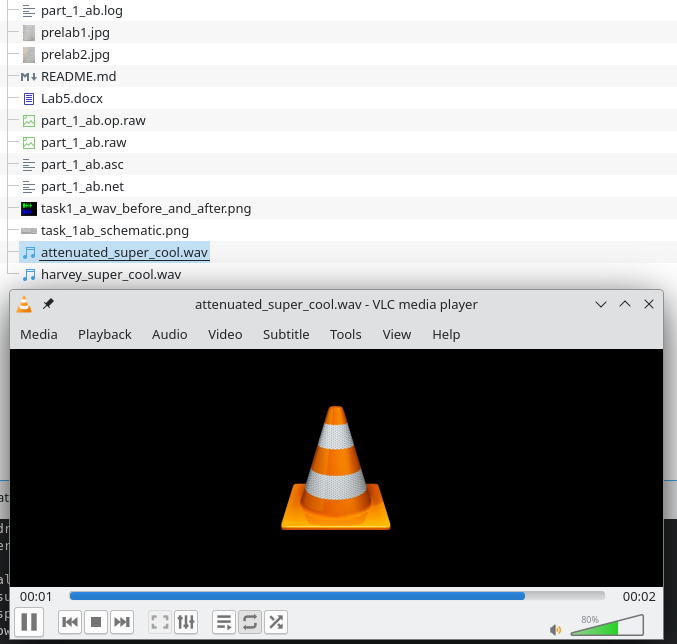
\includegraphics[width=0.85\linewidth]{task_1_b_play_attenuated}
		\caption{Playing the attenuated output audio}
		\label{fig:T1_PA_PLAYER}
		\vspace{1mm}
	\end{figure}


	\subsection{Part c: CS Stage Schematic}
	
	\subsubsection{Tasks}
	\begin{itemize}
		\item Use the values from prelab part (b) to create an LTSpice schematic for the CS Stage
	\end{itemize}
	
	\subsubsection{Description}
		The schematic was created using the values from Figure(\ref{fig:prelab1}), and an arbitrary choice of capacitance of $100uF$ for the input and output capacitors. The resulting schematic can be seen in Figure(\ref{fig:T1_PC_SCHEMATIC}).
		
		Then LTSpice tries to find an initial operating point value at the output capacitor for purposes of running the transient analysis, there is a short period where the output voltage would not be centered around $0V$. The addition of a $1M_\omega$ resistor on the output suppresses this effect.
		
	\begin{figure}[h]
		\centering
		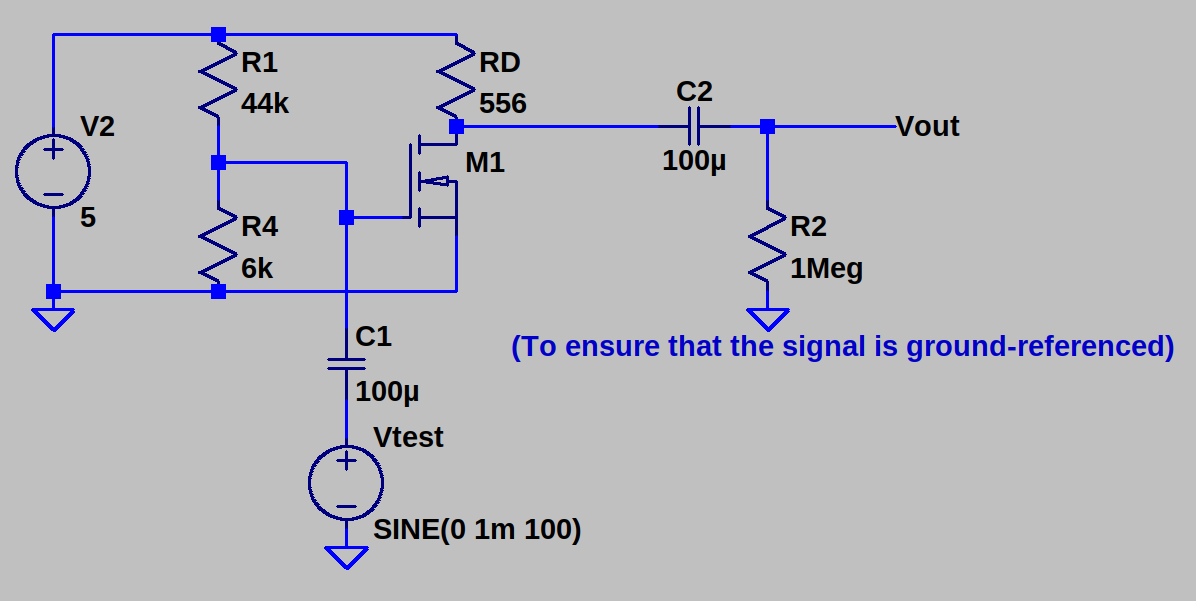
\includegraphics[width=0.85\linewidth]{task_1_c-e_schematic}
		\caption{CS Stage W/Resistor Bias and Load, Schematic}
		\label{fig:T1_PC_SCHEMATIC}
		\vspace{1mm}
	\end{figure}
	
	\subsection{Part d: CS Stage Operating Point}
		\subsubsection{Tasks}
		\begin{itemize}
			\item Run a .op analysis and verify the operating point matches our expectations from the prelab
		\end{itemize}
		
		\subsubsection{Description}
		We ran the .op analysis, the results of which are in Figure(\ref{fig:T1_PD_OP}). The key values to compare with the prelab in Figure(\ref{fig:prelab1}) are as follows:
		\begin{itemize}
			\item $V_g = 0.6V$ Matches the .op value of $V_\text{(n003)} = 0.6V$
			\item $I_d = 900\mu A$ Matches the .op value of $Id_\text{(M1)} = 0.0009V$
			\item Gate bias current of $100\mu A$ matches .op value of $I_\text{(R1)} = 0.0001V$
			\item Total Current of $1mA$ matches .op value of $I_\text{(V2)} = -.001 A$
		\end{itemize}
		
		Additionally, the spice error log (not shown) shows $g_m = 1.8e-02$, $V_{gs} = 6.00e-01$, and $V_{ds} = 4.5e+00$. These values are all exactly what is expected from the prelab calculations.
		
	\begin{figure}[h]
		\centering
		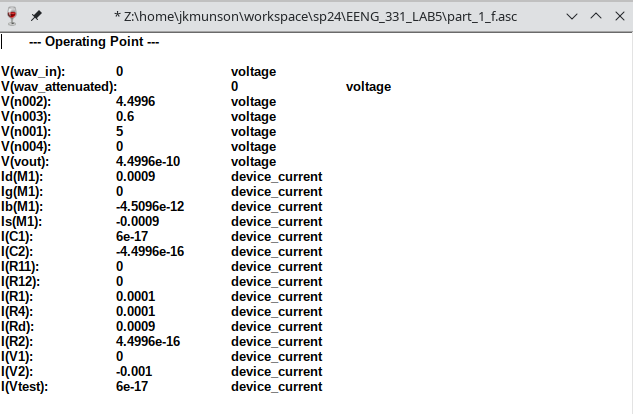
\includegraphics[width=0.85\linewidth]{task_1_d_operating_point}
		\caption{CS Stage W/Resistor Bias and Load, Operating Point Analysis}
		\label{fig:T1_PD_OP}
		\vspace{1mm}
	\end{figure}
	
	\subsection{Parts e, f: CS Stage .tran Test w/ 1mv sin and audio}
		\subsubsection{Tasks}
		\begin{itemize}
			\item Run a .tran simulation and verify the operation of the amplifier with a 1mv sine wave at 100hz
			\item Run a .tran simulation using the attenuated audio file as input and verify the circuit operation.
		\end{itemize}
	
		\subsubsection{Description}
			The $1mv$ input was fed into the device in a transient analysis, and the waveforms compared in Figure(\ref{fig:T1_PE_SIN}). A gain of $|A_V| = 10$ is observed, with an amplitude reversal because this is an inverting amplifier. This matches our calculated values for gain in the prelab when we include the amplitude reversal for an inverting amplifier. 
			
			The amplitude reversal could be seen as a $180\deg$ phase shift for the pure, periodic sine wave, but phase shifting implies time-shifting as well. If a signal containing multiple components or that was aperiodic were to be fed into a black box with "180 degree phase shift" on the sticker, then the result would be different than simple amplitude reversal. For this reason we prefer not to characterize this as a "phase shifting" action.
			
			Next, we changed the input over to the attenuated audio file from the previous parts of this task. The resulting waveforms can be seen in Figure(\ref{fig:T1_PF_WAV}). The audio is re-amplified from $\approx \pm 5mV$ to $\approx \pm 50mv$, demonstrating that the amplifier worked exactly as expected. It is also worth noting that the amplitude has in fact been reversed between the input and output; this can be observed by looking closely at the peaks in the figure, as the waveform is not symmetrical about 0v.
			
			Overall, the amplifier performed exactly as expected.
	\begin{figure}[h]
		\centering
		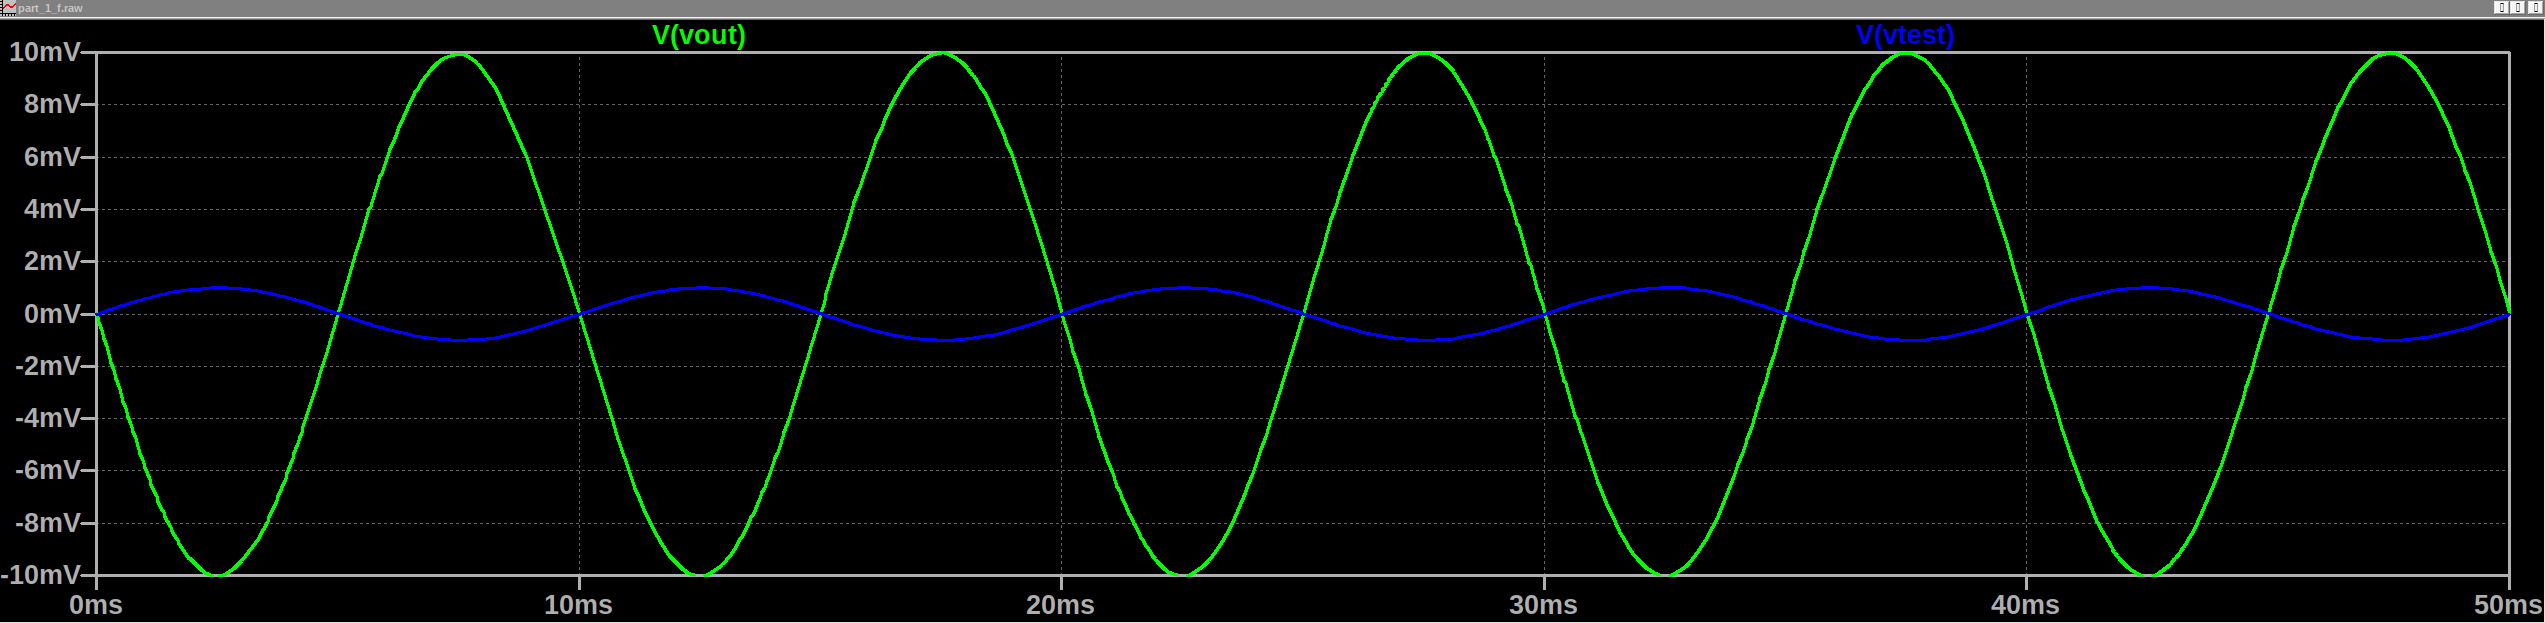
\includegraphics[width=0.95\linewidth]{task_1_e_waveform_av10}
		\caption{CS Stage W/Resistor Bias and Load, test with 1mv input}
		\label{fig:T1_PE_SIN}
		\vspace{1mm}
	\end{figure}

	\begin{figure}[h]
		\centering
		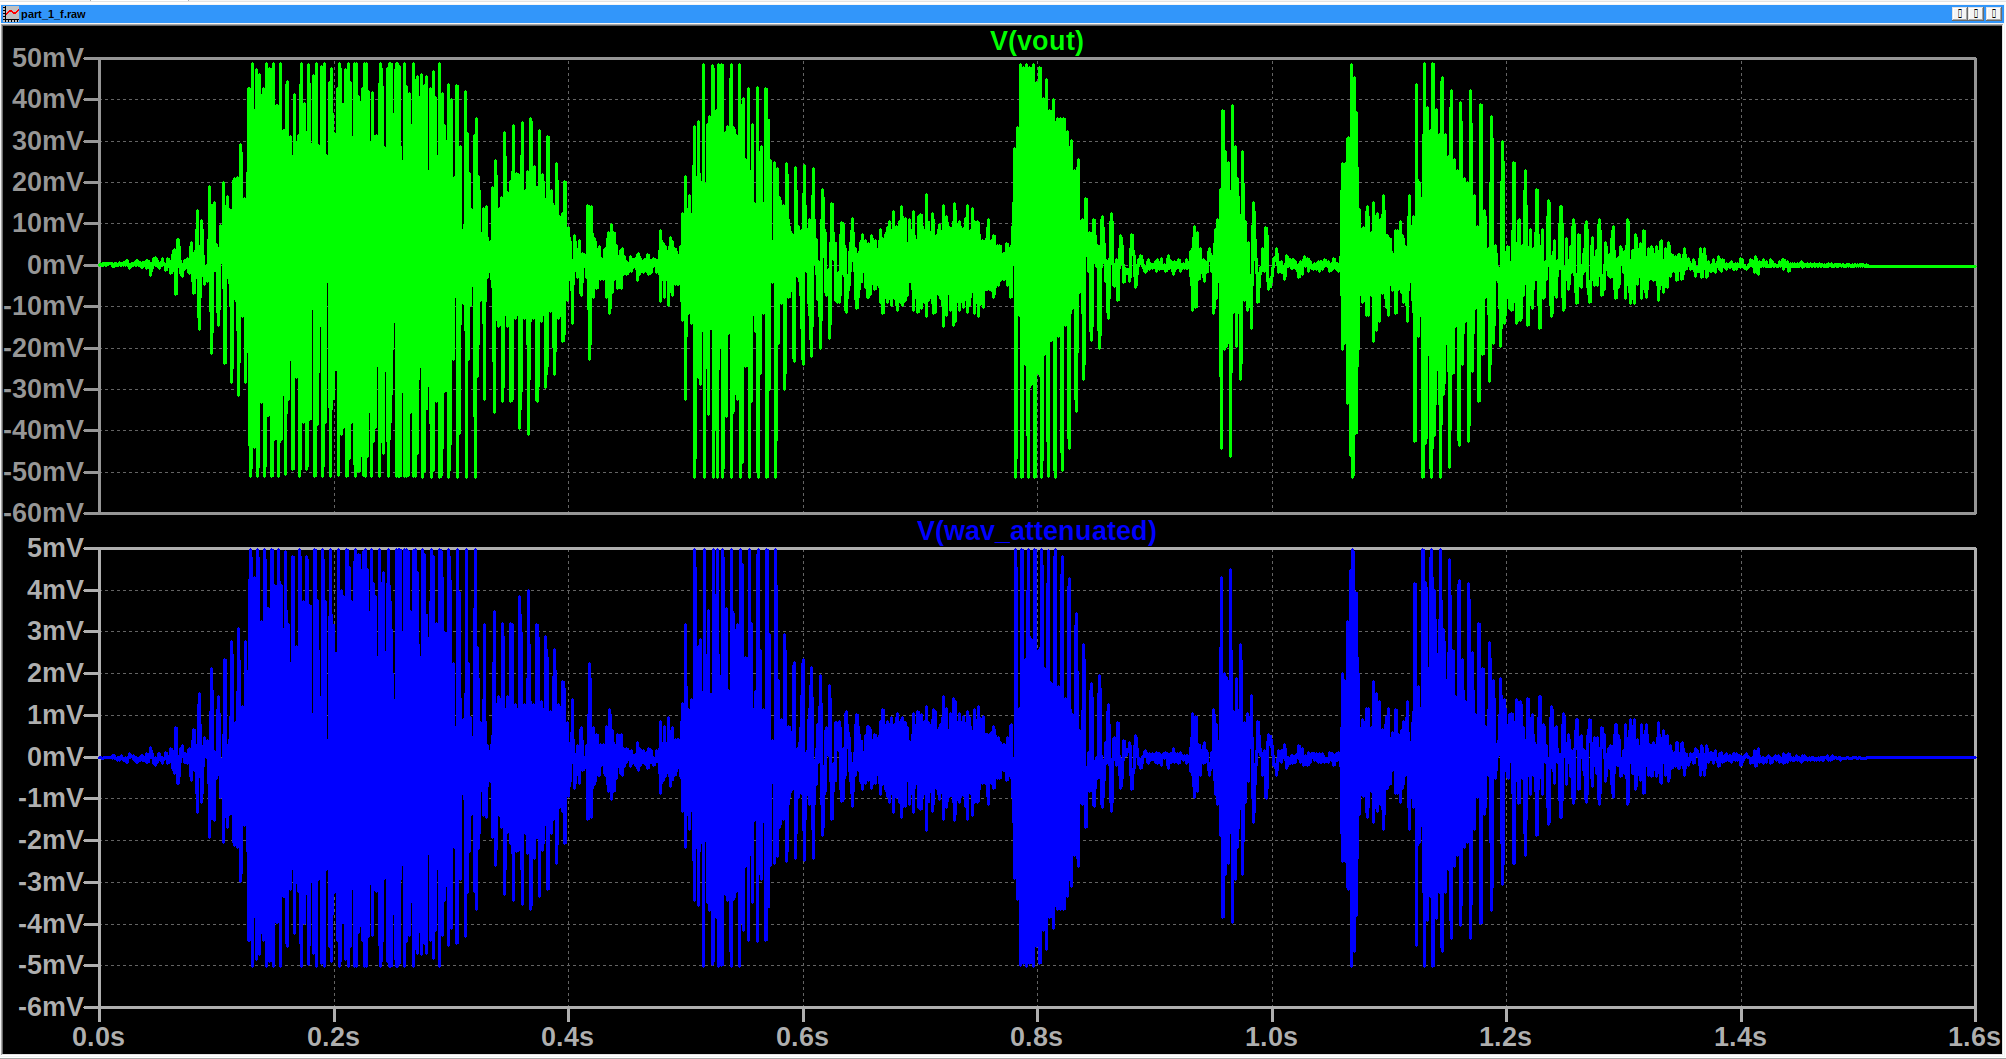
\includegraphics[width=0.95\linewidth]{task_1_f_amplify_the_attenuated_wav}
		\caption{CS Stage W/Resistor Bias and Load, re-amplify the audio}
		\label{fig:T1_PF_WAV}
		\vspace{1mm}
	\end{figure}

	\subsection{Part g: Increasing input impedance}
	\begin{itemize}
		\item Increase the input impedance of the design to $100k_\Omega$
		\item Verify that the design still works.
	\end{itemize}

	\subsection{Calculations}
		The increase the input impedance, we can increase the values of the resistors forming the biasing resistor divider. The current input impedance is given by Equation(\ref{eqn:T1_PG_impedance_before}):
		
		\begin{align}\label{eqn:T1_PG_impedance_before} R_{in} = (R_1^{-1} + R_2^{-1})^{-1} = (44000_\Omega^{-1} + 6000_\Omega^{-1})^{-1} = 5280_\Omega \end{align}
		
		If we don't bother to change the rest of the amplifier circuit design, then we will come in at a lower current, and lower overall power consumption. The difference is minor, so we simply adjust the voltage divider here. 
		
		The easiest way to increase the impedance will be to scale the voltage divider: Increase each resistor by a fixed factor. To do this, we write the ratio in Equation(\ref{eqn:T1_PG_impedance_ratio}):
		
		\begin{align}\label{eqn:T1_PG_impedance_ratio} 
			\frac{R_{in_{\text{after}}}}{R_{in_{\text{before}}}} = \frac{100000}{5280} \rightarrow R_{\text{after}} = R_{\text{before}}\cdot \frac{10000}{528}
		\end{align}
		
		Which results in $R_1 = 833333\Omega$ and $R_2 = 113636\Omega$.
		
		We make those value changes, and plot the resulting waveform in Figure(\ref{fig:T1_PG_ALL}). It can be seen that the amplifier still has a gain of $A_v = -10$ and functions exactly the same as before.
		
		\begin{figure}[h]
			\centering
			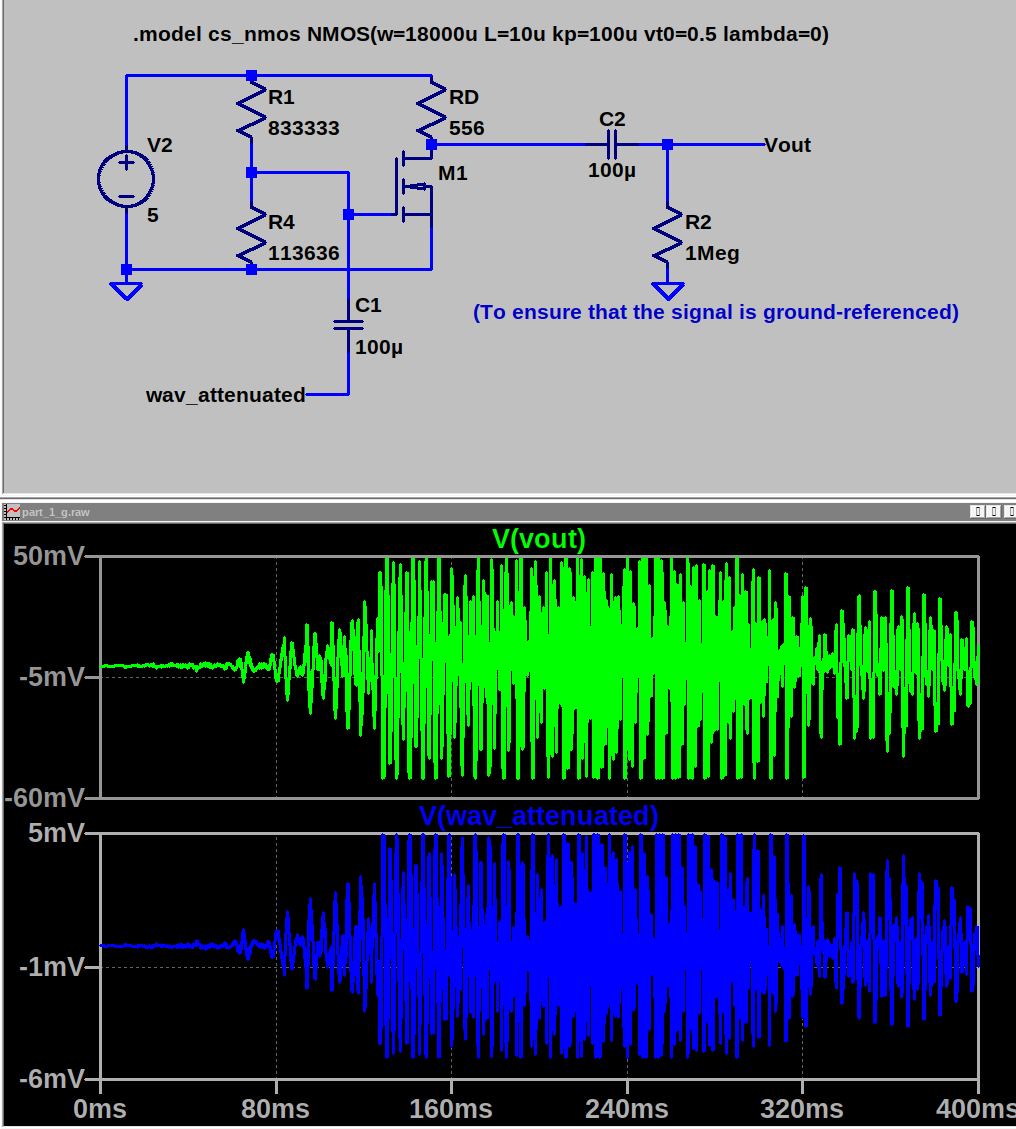
\includegraphics[width=0.85\linewidth]{task_1_g_easy_soln}
			\caption{CS Stage W/input impedance increased.}
			\label{fig:T1_PG_ALL}
			\vspace{1mm}
		\end{figure}
	
	\subsection{Part h: Can the gain be increased to 200?}
		We are asked if the gain of the amplifier could be increased to 200. The answer is "Yes, but". First, we address the "yes".
		
		The gain of the amplifier is used to calculate $R_D$ in Equation(\ref{eqn:CS_RD}). The gain is the product of $R_D$ and $g_m$. Our $g_m$ is fixed if we keep the same power budget, but we can increase $R_D$ without limit. For this reason, we can make the gain arbitrarily large, including a value of 200.
		
		Now, for the "no": The gain is limited by the channel modulation effects in a real mos device. The gain for a real mos device would be given by Equation(\ref{eqn:T1_PF_REAL_GAIN}):
		\begin{align}\label{eqn:T1_PF_REAL_GAIN} 
			A_v = g_m\cdot(R_D \parallel r_o)
		\end{align}
		So we see that as we increase $R_D$, eventually we get Equation(\ref{eqn:T1_PF_REAL_GAIN2}):
		\begin{equation} 
			\lim_{R_D \to \infty}...,\text{\quad}
			A_V = g_m\cdot r_o \label{eqn:T1_PF_REAL_GAIN2}
		\end{equation}
	So the overall gain would be limited by the value of $r_o$, which is proportional to $\lambda$. For $\lambda \neq 0$, we may or may not be able to reach a gain of 200. In other words, with real mos devices we are limited to the intrinsic gain of the device.
	
	From a different angle, If the gain were 200 then we would clip our audio signal. Since $V_{ds\text{,dc}} = 4.5V$, we have significantly less headroom than would be needed for the $\pm 1V$ output.
		
		
	\FloatBarrier
	%\quad 
	\newpage
	\addcontentsline{toc}{section}{Table Of Contents}
	\setcounter{tocdepth}{2}
	\begin{spacing}{0.1}
		\tableofcontents
		\listoffigures
	\end{spacing}

\end{document}